% Diplomarbeit deutsch Matthias Kreier
% weitere Informationen unter http://people.physik.hu-berlin.de/~kreier/

\documentclass[11pt,twoside,german]{book}
%\nofiles % verhindert Ausgabe einer neuen TOC
\usepackage{palatino}
\usepackage[OT2,T1]{fontenc}
\usepackage{ucs}
\usepackage[utf8x]{inputenc}
\usepackage{geometry}
\geometry{verbose,a4paper,tmargin=35mm,bmargin=25mm,lmargin=25mm,rmargin=25mm,headheight=10mm,headsep=10mm,footskip=10mm}
\pagestyle{headings}
\setcounter{secnumdepth}{3}
\setcounter{tocdepth}{3}
\usepackage{graphicx}
\usepackage{amsmath}
\usepackage{amssymb}
\usepackage[russian,ngerman]{babel}
\newcommand\ru[1]{\foreignlanguage{russian}{#1}}  % um russische Texte einzubinden
%\usepackage{ae}   % Die Umlaute werden dann wieder unschön, das ß geht verloren ... (in Palatino)
\usepackage[pdftex,pdfpagelabels=true]{hyperref}
%\usepackage[pdftex]{thumbpdf}

\makeatletter
  \newcommand{\noun}[1]{\textsc{#1}}

  \DeclareRobustCommand*\textsubscript[1]{%
    \@textsubscript{\selectfont#1}}
  \newcommand{\@textsubscript}[1]{%
    {\m@th\ensuremath{_{\mbox{\fontsize\sf@size\z@#1}}}}}

  \renewcommand{\chaptermark}[1]{%
  \markboth{#1}{}}
  \renewcommand{\sectionmark}[1]{%
  \markright{#1}{}}

% \bibliographystyle{Nplain} % Stil der Phys. Rev. Ausgaben ist amsplain
\hypersetup{%
 colorlinks=true,
 linkcolor=blue,
 citecolor=blue,
 pdftitle	= {Electronic Properties of CdHgTe},
 pdfsubject	= {Diplomarbeit Institut für Physik},
 pdfauthor	= {Matthias Kreier},
 pdfkeywords	= {ARPES,CdHgTe},
 pdfcreator	= {Adobe-Acrobat-Distiller},
 pdfproducer	= {LaTeX with hyperref and thumbpdf}
}
\makeatother

\begin{document}
\frontmatter
\pagenumbering{Roman}
\begin{titlepage}
\begin{center}
\vspace*{2mm}
{\Huge
Elektronische Struktur der\\
ternären II/VI-Halbleiter\\[1.2mm]
Cd\textsubscript{\large1-X}Hg\textsubscript{\large X}Te}\\[13mm]
{\Large Diplomarbeit}\\[20mm]
\includegraphics[ width=40mm, height=40mm]{pic/husiegel_bw_rgb}\\[20mm]
\noun{
Humboldt-Universität zu Berlin\\
%Mathematisch-Naturwissenschaftliche Fakultät I\\
Institut für Physik\\
AG Elektronische Eigenschaften und Supraleitung}\\[15mm]
eingereicht von\\[10mm]
{
Matthias Kreier\\
geb. am 3.10.1975 in Nauen}\\[15mm]
\end{center}
1. Gutachter: Professor Recardo Manzke\\[3mm]
2. Gutachter: Prof. \\[3mm]
Berlin, 25. 1. 2008
\end{titlepage}

\setcounter{page}{0}

\tableofcontents{}

\mainmatter

\chapter{Einleitung}

The field of semiconductors has undergoing a big process of whatsoever. In former 
times the II-VI-Semiconductors were higly estimated and ... 

\ru{Добрый день, Добро пожаловать в \LaTeXе!}

Even in the late 1970s Cd HgTe has been estimated and analyzed with electrons, photons and 
of course neutrons.

The crystals of HgTe and PbTe as well as CdTe and SnTe have been studied
during the last tree decades very intensively. Whereas the first two
are considered to be narrow bandgap \cite{hertz} semiconductors the latter two
are semimetals. CdTe shows an inverted bulk bandstructure and has
therefore a negative bandgap.

Here I describe in two sentences the content of each chapter \cite{theorie1}.
At least one citation will be included.


The Fermi level lies between them in the gap \cite{shirley} and the oxide is an insulator.
Both the ionic picture and the band theory are valid. The electronic excitation
of lowest energy determines the gap width shown in Figure \ref{fermikante}. In
this case, this is a charge-transfer excitation\footnote{excitation = Anregung}
and corresponds to the transfer of an electron
from the anion to the cation. The charge-transfer energy is denoted. In a
partially occupied shell system, however, the oxide may be insulating though
the band theory predicts a metallic state. This is because the representation
of the repulsion between electrons by an average effective potential is not a
good approximation anymore when electron correlation becomes important.
This term describes the way electrons move in order to avoid each other and
to the interatomic overlap. At a critical value around W (band width) 
U, the upper and lower states overlap and the gap vanishes [5]. Zaanen et
al. have classified the insulators using both parameters  and U in a phase
diagram [17]. For a Mott-Hubbard insulator where E\textsubscript{gap} / U , both
holes and electrons move in d bands and are heavy, while.

Et nostrud delicatissimi mea, zzril aeterno ocurreret ut ius. Ius elitr adipisci gloriatur ad, vero augue graece ei nam. Et qui facilisis gloriatur scribentur, usu viris blandit expetenda eu. Sed ad eligendi legendos posidonium, et nostro intellegam vis. In nominati temporibus scriptorem vel. Ne cum takimata periculis definiebas, et inani zzril consequuntur mei, sit ei feugait hendrerit.

Prompta complectitur ad sit, at eligendi oporteat deserunt eum. At duo puto commodo necessitatibus, mei nobis iisque aliquam ea. Duo cu oblique vivendo corrumpit. Ea dicat ubique alterum nam.

Altera deterruisset eum eu, ne vix commodo partiendo democritum. Mel ut sint vulputate. Aperiri postulant mei cu, ius at atqui graeci salutatus. Id tale hinc sapientem eum, ad eum quod adhuc. Te sit sint accusam.

Ex quem apeirian deseruisse nam, qui eu odio moderatius, augue sensibus erroribus te eum. Accusam adversarium definitionem an has, puto fabulas ne sed, an mel mazim malorum. Eam ne verear reformidans. Scaevola expetenda ei vel, sensibus mediocrem dignissim id usu, dictas verear suavitate mei ad. Nec ad definiebas disputando. Debitis habemus alienum in mea, menandri posidonium an mel.

Vim quod voluptua cu. Veniam dicunt id mei. Primis perpetua mei eu, tibique concludaturque ad sea. Kasd pertinacia qui eu, ex deserunt neglegentur ius. Perpetua scribentur contentiones no mel, ei mel probatus singulis patrioque, eu modus patrioque definitiones quo.

Omnes congue ad quo, ad dicat nonummy sit. Pri an amet consulatu, scaevola vivendum no usu. Ea usu commune torquatos liberavisse. Ius quot duis signiferumque no.

Eos suscipit posidonium reprimique ne, nec forensibus comprehensam cu. Nec in sint aeterno sapientem, sea cu nonumy vidisse impedit. Te libris torquatos reprehendunt sea. Ea cum perpetua petentium intellegebat, oratio labore ceteros eu pri. Veniam gubergren contentiones est id.

Modus invenire persecuti eu sit, dolor doming accusamus nec ei. Atqui explicari ea pro, at eos veri integre mentitum. Eu has assum nobis nominati. Nec ex suas scripserit. Quem magna cotidieque no sit. An esse iuvaret cotidieque eam, ne nulla aeque molestiae nec, virtute appareat quaestio an eos.

Finally this chapter ends.

\chapter{Grundlagen der winkelaufgelösten Photo Elektron Spektroskopie}
\section{Meßprinzip}

To study the electronical properties of a material we use the photoelectric effect, that is
the emission of electrons upon the absorption of electromagnetic radiation. This effect was 
discovered by Heinrich Hertz (1886 Hertz effect, \cite{hertz}) and his assistant Wilhelm Hallwachs 
(1887 Hallwachs effect, \cite{hallwachs}). Max Planck published in 1901 his law of radiation. He went on 
to state that the energy lost or gained by an oscillator is emitted or absorbed as a quantum 
of radiant energy, the magnitude of which is expressed by the equation:

\[E=h\nu\]

E equals the radiant energy, h is Planck's constant and $\nu$ is the frequency of radiation. 
In 1905 Albert Einstein applied Planck's theory and explained the photoelectric effect in terms of 
the quantum model using his famous equation for which he received the Nobel Prize in 1921:

\begin{equation}
E_{kin}^{max}=h\nu - \Phi
\end{equation}

The maximum kinetic energy $E_{kin}$ of the emitted photoelectrons equals the photon energy $h\nu$ minus the 
energy $\Phi$ needed to remove them from the surface of the material. This binding energy  $\Phi$ is 
also called the work function. The inverse relation to [Gleichung von ebenda] exists between the maximum 
energy of the Xray radiation and the electron energy the matter is irradiated.

Angle resolved - why ... ARPES
If photon is UV it is called UPS or UVPES and XPS for x-ray.


\[E=mc^{2}\]

As you can see, the intensity not only depends on the wavefunction of the incomming light but due to the vector potential to the azimuth and polar angle. This is discovered by an spherical analysator (Scienta SES 100) with a multichannel plate.

\[\Delta E=1/2E_{PASS}+\alpha\]

This formulae is obtained by a single integration of all amplitude
data measured within a certain period. Later recalculated intensity
revitalises all dependencies. 

Here follows a little text with no meaning, only to get to page ..
next .. and there I need a little paragraph.

Maybe this is my paragraph, I hope I'll like him. Here now a picture
is to be introduced. Let's see if it figures out.


\section{Prozess der Photoemission und Untersuchung der Bandstruktur}

While the photo emission is as easy and then later and here a text.
I'll try to impact a formulae in this text with Lyx so let's see if
it works: $2k_{B}T=25meV$ sollte mit Subs funktionieren. Probieren
wir es gleich noch einmal.

\[E_{k}=\sin(\beta+\pi/4)\]

$\vec{E=1/2\sin a}$ und so geht der Text weiter. ein $\vec{E}=\frac{1}{2}mv^{2}$und
so geht die english translation further and further. Keep on thinking
about it. Maybe it helps. See you tomorrow. As for me - I can't go
on living like that and pretend that everything is ok. Therefore don't
ask, just read.

As for the bandstructure one obtains various many-body-effects on
the surface. Usually described as a thin layer, it is not nessesaryly
a big deal. Watch this formulae:
\begin{eqnarray*}
E_{f} & = & E_{gap}+E_{Austrittsarbeit}+k_{b}T^{1/2}
\end{eqnarray*}


Not linear dependant it perfectly shows nothing.

Fitting parameters are not avaliable. Suiting 4 Gauss profiles leed
to an extraordinary dispersion in light intensity:

\begin{center}
\begin{tabular}{|c|c|c|c|}
\hline 
photon energy&
kink at {[}eV{]}&
vec&
transmission\tabularnewline
\hline
\hline 
22.12&
3.546&
12.1&
14.3\tabularnewline
\hline 
22.12&
6.543&
12.4&
35.3\tabularnewline
\hline
\end{tabular}
\end{center}

The slight shift in intensity is connected to the thin bilayer splitting
in HTSC based on YBCO. Bi2212 dosn't shows this behavior.

Et nostrud delicatissimi mea, zzril aeterno ocurreret ut ius. Ius elitr adipisci gloriatur ad, vero augue graece ei nam. Et qui facilisis gloriatur scribentur, usu viris blandit expetenda eu. Sed ad eligendi legendos posidonium, et nostro intellegam vis. In nominati temporibus scriptorem vel. Ne cum takimata periculis definiebas, et inani zzril consequuntur mei, sit ei feugait hendrerit.

Prompta complectitur ad sit, at eligendi oporteat deserunt eum. At duo puto commodo necessitatibus, mei nobis iisque aliquam ea. Duo cu oblique vivendo corrumpit. Ea dicat ubique alterum nam.

Altera deterruisset eum eu, ne vix commodo partiendo democritum. Mel ut sint vulputate. Aperiri postulant mei cu, ius at atqui graeci salutatus. Id tale hinc sapientem eum, ad eum quod adhuc. Te sit sint accusam.

Prompta complectitur ad sit, at eligendi oporteat deserunt eum. At duo puto commodo necessitatibus, mei nobis iisque aliquam ea. Duo cu oblique vivendo corrumpit. Ea dicat ubique alterum nam.

Altera deterruisset eum eu, ne vix commodo partiendo democritum. Mel ut sint vulputate. Aperiri postulant mei cu, ius at atqui graeci salutatus. Id tale hinc sapientem eum, ad eum quod adhuc. Te sit sint accusam.
\newpage

\begin{figure}
\begin{center}
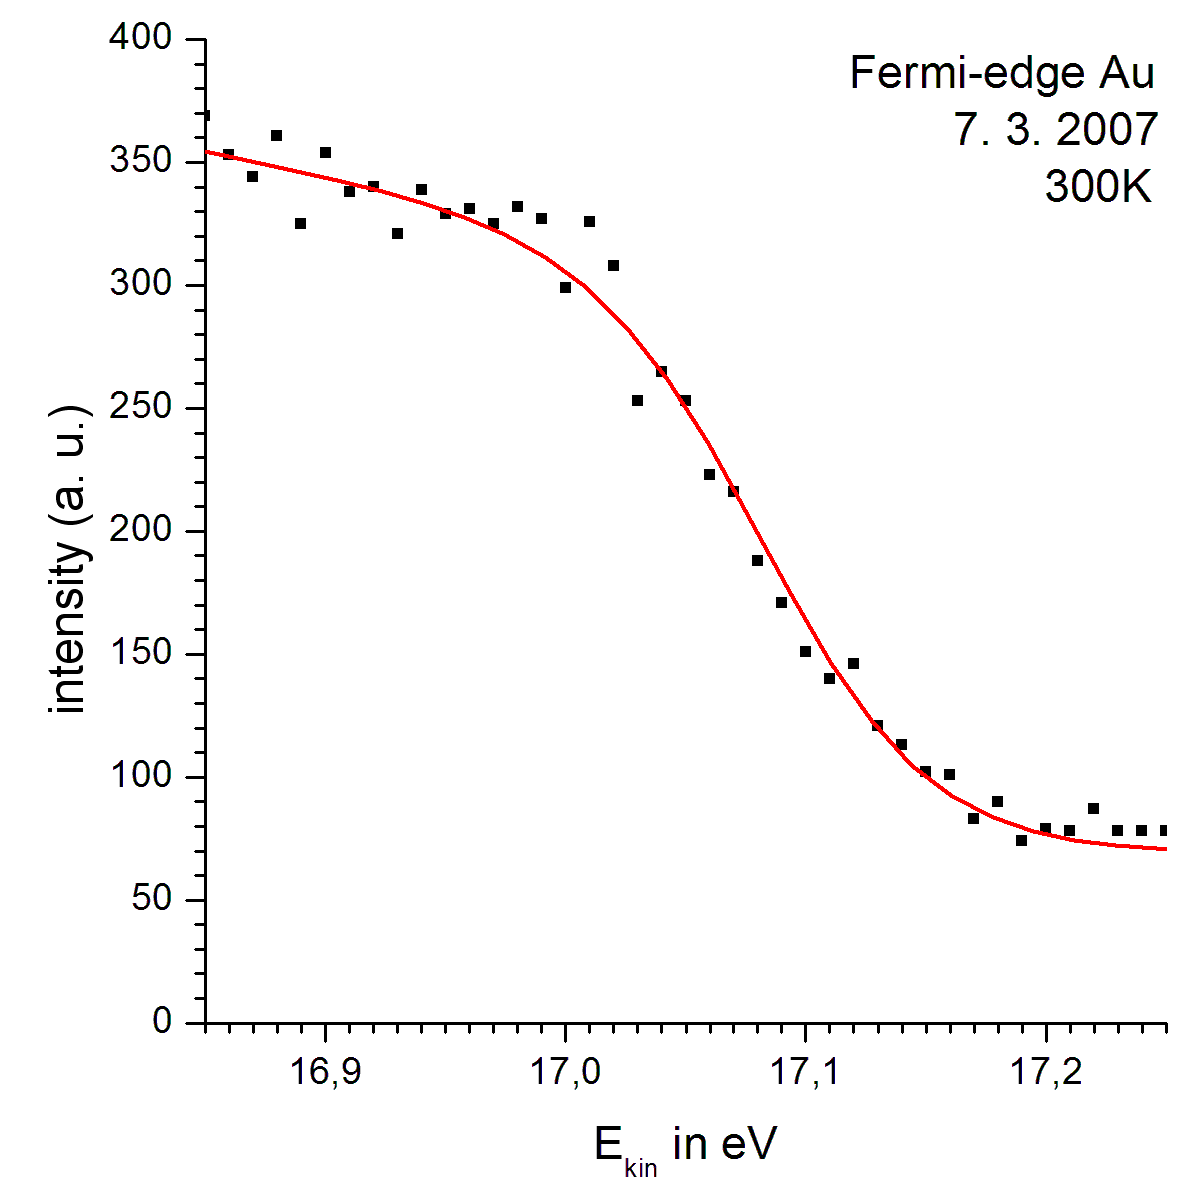
\includegraphics[width=100mm, keepaspectratio]{pic/fermikante}
\caption{\label{fermikante}Aufbau der Meßkammer}
\end{center}
\end{figure}

1,5 mGauß nachgewiesen(vgl. Erdmagnetfeld: max 500 mGauß). Wichtig für die Experimente ist die Unterteilung der Kammer in mehrere Ebenen: Transferebene, Zusatzebene, Meßebene und Pumpebene (von oben nach unten, siehe auch Abb. 3.2 und 3.1) In der Transferebene können die Proben eingeschleust, manipuliert und orientiert werden. Der Probentransfer zwischen Probenschleuse und Meßkammer wird mit einer sog. Transferstange realisiert, die mit einem speziellen Gabelkopf zur Aufnahme der Probenhalter ausgerüstet wurde (zu den Probenhaltern siehe Kap. 5.5) Der Kryostat, der von oben auf die Kammer aufgesetzt ist, nimmt die Proben auf. In die Transferebene wurde ein Vakuum-Manipulierarm (engl. {\it wobble stick}) eingebaut, um bestimmte Arbeitsgänge im Vakuum, zum Beisiel das Betätigen der Kühlschildklappe (Kap. 3.5) oder das Abreißen der Spalthebel (siehe Kap. 5.5), zu ermöglichen. Mit der Zweitrotation des Kryostaten, d.h. die Rotation um die Probennormale, können die Proben optimal orientiert werden.

Ebenfalls wurde in diese Ebene ein LEED/Auger-System (Kap. 3.4) eingebaut. Dadurch können strukturelle wie chemische Eigenschaften der Proben in situ untersucht werden. Insbesondere kann die Probenorientierung durch LEED überprüft werden. Ist die Probe einmal orientiert, wird sie mit dem Kryostaten in die untere Ebene, die Meßebene, gefahren. In der Meßebene fallen (ein genau einjustiertes Experiment vorausgesetzt) der Fokus der Synchrotronstrahlung aus dem Monochromator und 
\newpage

Ex quem apeirian deseruisse nam, qui eu odio moderatius, augue sensibus erroribus te eum. Accusam adversarium definitionem an has, puto fabulas ne sed, an mel mazim malorum. Eam ne verear reformidans. Scaevola expetenda ei vel, sensibus mediocrem dignissim id usu, dictas verear suavitate mei ad. Nec ad definiebas disputando. Debitis habemus alienum in mea, menandri posidonium an mel.

Vim quod voluptua cu. Veniam dicunt id mei. Primis perpetua mei eu, tibique concludaturque ad sea. Kasd pertinacia qui eu, ex deserunt neglegentur ius. Perpetua scribentur contentiones no mel, ei mel probatus singulis patrioque, eu modus patrioque definitiones quo.

Omnes congue ad quo, ad dicat nonummy sit. Pri an amet consulatu, scaevola vivendum no usu. Ea usu commune torquatos liberavisse. Ius quot duis signiferumque no.

\section{Oberflächenzustände und Bulkbandstruktur}

Eos suscipit posidonium reprimique ne, nec forensibus comprehensam cu. Nec in sint aeterno sapientem, sea cu nonumy vidisse impedit. Te libris torquatos reprehendunt sea. Ea cum perpetua petentium intellegebat, oratio labore ceteros eu pri. Veniam gubergren contentiones est id.

Ad omnis habeo antiopam eam, partem insolens sit et, eam enim appareat conceptam eu. Vocent inimicus neglegentur quo ad, ad nec etiam interpretaris, ex wisi idque regione nec. Pri ut quas nostrum, velit civibus ne sit. Sea simul feugiat cu, te alii invenire consectetuer nam, vim ad contentiones sonet vituperatoribus.

\section{Unterschiedliche Modi der Photo Emissions Spektroskopie (EDC, XDC)}

Civibus eleifend definitionem mel ei, placerat perfecto et qui. Eam cu quas mundi volumus. Ius quidam theophrastus ne, te mea viris dissentias. Et vis homero nominavi ocurreret. No has audiam invidunt percipitur, mei esse aliquam epicuri id. Omnes nominati forensibus in per, in eam tempor periculis constituam.

Modus invenire persecuti eu sit, dolor doming accusamus nec ei. Atqui explicari ea pro, at eos veri integre mentitum. Eu has assum nobis nominati. Nec ex suas scripserit. Quem magna cotidieque no sit. An esse iuvaret cotidieque eam, ne nulla aeque molestiae nec, virtute appareat quaestio an eos.

\chapter{Grundlegendes über II-VI Halbleiter}

\section{Kristallstruktur, Volumen-Brilloinzone}

All measurements were taken with the SCIENTA SES 100 and the WESPHOA
I at the laboratry in Adlershof, Newtonstr. 14. Very usefull for interpretration
of the mesurement data was all GPL-software and so on.

Ex quem apeirian deseruisse nam, qui eu odio moderatius, augue sensibus erroribus te eum. Accusam adversarium definitionem an has, puto fabulas ne sed, an mel mazim malorum. Eam ne verear reformidans. Scaevola expetenda ei vel, sensibus mediocrem dignissim id usu, dictas verear suavitate mei ad. Nec ad definiebas disputando. Debitis habemus alienum in mea, menandri posidonium an mel.

\section{Oberflächenzustände}

Eos suscipit posidonium reprimique ne, nec forensibus comprehensam cu. Nec in sint aeterno sapientem, sea cu nonumy vidisse impedit. Te libris torquatos reprehendunt sea. Ea cum perpetua petentium intellegebat, oratio labore ceteros eu pri. Veniam gubergren contentiones est id.

Ad omnis habeo antiopam eam, partem insolens sit et, eam enim appareat conceptam eu. Vocent inimicus neglegentur quo ad, ad nec etiam interpretaris, ex wisi idque regione nec. Pri ut quas nostrum, velit civibus ne sit. Sea simul feugiat cu, te alii invenire consectetuer nam, vim ad contentiones sonet vituperatoribus.

\chapter{Elektronische Eigenschaften von CdTe, HgTe und Cd$_{1-X}$Hg$_{X}$Te}
\markright{\upshape Elektronische Eigenschaften von CdTe, HgTe und Cd$_{1-X}$Hg$_{X}$Te}
\section{Halbleiter mit schmaler Bandlücke}

In the late 60s the first time appeard the word 'zero bandgap semiconductor' whereas the question arises what a zero gap should be. Soon thereafter an new word was used for HgTe: a semiconductor with 'negative bandgap'. To illustrate the meaning of this, please look at fig. 1 and 2 to distinquish betweet both core levels.

effective potential is not a
good approximation anymore when electron correlation becomes important.
This term describes the way electrons move in order to avoid each other and
has to be taken into account especially in very narrow bands. The Hubbard
model describes this insulating state introducing the Hubbard energy
U. This is the energy U required for the exchange of an electron between
two cations, yielding the formation of two bands: the lower and the upper
Hubbard sub-bands. The correlation competes with the delocalization due

\section{Theoretische Bandstruktur}

Et nostrud delicatissimi mea, zzril aeterno ocurreret ut ius. Ius elitr adipisci gloriatur ad, vero augue graece ei nam. Et qui facilisis gloriatur scribentur, usu viris blandit expetenda eu. Sed ad eligendi legendos posidonium, et nostro intellegam vis. In nominati temporibus scriptorem vel. Ne cum takimata periculis definiebas, et inani zzril consequuntur mei, sit ei feugait hendrerit.

Prompta complectitur ad sit, at eligendi oporteat deserunt eum. At duo puto commodo necessitatibus, mei nobis iisque aliquam ea. Duo cu oblique vivendo corrumpit. Ea dicat ubique alterum nam.

Altera deterruisset eum eu, ne vix commodo partiendo democritum. Mel ut sint vulputate. Aperiri postulant mei cu, ius at atqui graeci salutatus. Id tale hinc sapientem eum, ad eum quod adhuc. Te sit sint accusam.

Therefore we need the GW-approximation! Here it comes: see you ....

The Hubbard
model describes this insulating state introducing the Hubbard energy
U. This is the energy U required for the exchange of an electron between
two cations, yielding the formation of two bands: the lower and the upper
Hubbard sub-bands. The correlation competes with the delocalization due
to the interatomic overlap. At a critical value around W (band width) 
U, the upper and lower states overlap and the gap vanishes [5]. Zaanen et
al. have classified the insulators using both parameters  and U in a phase


\chapter{Experimenteller Aufbau}
\markright{\upshape experimentelle Methoden und Ausrüstung}
\section{Zusammenbau}

Et nostrud delicatissimi mea, zzril aeterno ocurreret ut ius. Ius elitr adipisci gloriatur ad, vero augue graece ei nam. Et qui facilisis gloriatur scribentur, usu viris blandit expetenda eu. Sed ad eligendi legendos posidonium, et nostro intellegam vis. In nominati temporibus scriptorem vel. Ne cum takimata periculis definiebas, et inani zzril consequuntur mei, sit ei feugait hendrerit.

Prompta complectitur ad sit, at eligendi oporteat deserunt eum. At duo puto commodo necessitatibus, mei nobis iisque aliquam ea. Duo cu oblique vivendo corrumpit. Ea dicat ubique alterum nam.

Altera deterruisset eum eu, ne vix commodo partiendo democritum. Mel ut sint vulputate. Aperiri postulant mei cu, ius at atqui graeci salutatus. Id tale hinc sapientem eum, ad eum quod adhuc. Te sit sint accusam.

\section{Vorbereitung der Proben}

Ex quem apeirian deseruisse nam, qui eu odio moderatius, augue sensibus erroribus te eum. Accusam adversarium definitionem an has, puto fabulas ne sed, an mel mazim malorum. Eam ne verear reformidans. Scaevola expetenda ei vel, sensibus mediocrem dignissim id usu, dictas verear suavitate mei ad. Nec ad definiebas disputando. Debitis habemus alienum in mea, menandri posidonium an mel.

Vim quod voluptua cu. Veniam dicunt id mei. Primis perpetua mei eu, tibique concludaturque ad sea. Kasd pertinacia qui eu, ex deserunt neglegentur ius. Perpetua scribentur contentiones no mel, ei mel probatus singulis patrioque, eu modus patrioque definitiones quo.

Omnes congue ad quo, ad dicat nonummy sit. Pri an amet consulatu, scaevola vivendum no usu. Ea usu commune torquatos liberavisse. Ius quot duis signiferumque no.

\section{Charakterisierung}

Eos suscipit posidonium reprimique ne, nec forensibus comprehensam cu. Nec in sint aeterno sapientem, sea cu nonumy vidisse impedit. Te libris torquatos reprehendunt sea. Ea cum perpetua petentium intellegebat, oratio labore ceteros eu pri. Veniam gubergren contentiones est id.

Ad omnis habeo antiopam eam, partem insolens sit et, eam enim appareat conceptam eu. Vocent inimicus neglegentur quo ad, ad nec etiam interpretaris, ex wisi idque regione nec. Pri ut quas nostrum, velit civibus ne sit. Sea simul feugiat cu, te alii invenire consectetuer nam, vim ad contentiones sonet vituperatoribus.

\subsection{Overflächenuntersuchung mit LEED}

Civibus eleifend definitionem mel ei, placerat perfecto et qui. Eam cu quas mundi volumus. Ius quidam theophrastus ne, te mea viris dissentias. Et vis homero nominavi ocurreret. No has audiam invidunt percipitur, mei esse aliquam epicuri id. Omnes nominati forensibus in per, in eam tempor periculis constituam.

Modus invenire persecuti eu sit, dolor doming accusamus nec ei. Atqui explicari ea pro, at eos veri integre mentitum. Eu has assum nobis nominati. Nec ex suas scripserit. Quem magna cotidieque no sit. An esse iuvaret cotidieque eam, ne nulla aeque molestiae nec, virtute appareat quaestio an eos.

\subsection{XPS und EDX Ergebnisse}

Eos suscipit posidonium reprimique ne, nec forensibus comprehensam cu. Nec in sint aeterno sapientem, sea cu nonumy vidisse impedit. Te libris torquatos reprehendunt sea. Ea cum perpetua petentium intellegebat, oratio labore ceteros eu pri. Veniam gubergren contentiones est id.

Ad omnis habeo antiopam eam, partem insolens sit et, eam enim appareat conceptam eu. Vocent inimicus neglegentur quo ad, ad nec etiam interpretaris, ex wisi idque regione nec. Pri ut quas nostrum, velit civibus ne sit. Sea simul feugiat cu, te alii invenire consectetuer nam, vim ad contentiones sonet vituperatoribus.

\subsection{Kristalluntersuchung mittels Laue-Verfahren}

Ex quem apeirian deseruisse nam, qui eu odio moderatius, augue sensibus erroribus te eum. Accusam adversarium definitionem an has, puto fabulas ne sed, an mel mazim malorum. Eam ne verear reformidans. Scaevola expetenda ei vel, sensibus mediocrem dignissim id usu, dictas verear suavitate mei ad. Nec ad definiebas disputando. Debitis habemus alienum in mea, menandri posidonium an mel.

Vim quod voluptua cu. Veniam dicunt id mei. Primis perpetua mei eu, tibique concludaturque ad sea. Kasd pertinacia qui eu, ex deserunt neglegentur ius. Perpetua scribentur contentiones no mel, ei mel probatus singulis patrioque, eu modus patrioque definitiones quo.


Ex quem apeirian deseruisse nam, qui eu odio moderatius, augue sensibus erroribus te eum. Accusam adversarium definitionem an has, puto fabulas ne sed, an mel mazim malorum. Eam ne verear reformidans. Scaevola expetenda ei vel, sensibus mediocrem dignissim id usu, dictas verear suavitate mei ad. Nec ad definiebas disputando. Debitis habemus alienum in mea, menandri posidonium an mel.

\chapter{Photoemission an Narrow-Gap-Halbleitern}

Vim quod voluptua cu. Veniam dicunt id mei. Primis perpetua mei eu, tibique concludaturque ad sea. Kasd pertinacia qui eu, ex deserunt neglegentur ius. Perpetua scribentur contentiones no mel, ei mel probatus singulis patrioque, eu modus patrioque definitiones quo.


Ex quem apeirian deseruisse nam, qui eu odio moderatius, augue sensibus erroribus te eum. Accusam adversarium definitionem an has, puto fabulas ne sed, an mel mazim malorum. Eam ne verear reformidans. Scaevola expetenda ei vel, sensibus mediocrem dignissim id usu, dictas verear suavitate mei ad. Nec ad definiebas disputando. Debitis habemus alienum in mea, menandri posidonium an mel.


\chapter{Die elektronische Struktur von CdHgTe}
\markright{\upshape Band Diagramm von II/VI Halbleitern}
\section{Allgemeine Ergebnisse}

Ex quem apeirian deseruisse nam, qui eu odio moderatius, augue sensibus erroribus te eum. Accusam adversarium definitionem an has, puto fabulas ne sed, an mel mazim malorum. Eam ne verear reformidans. Scaevola expetenda ei vel, sensibus mediocrem dignissim id usu, dictas verear suavitate mei ad. Nec ad definiebas disputando. Debitis habemus alienum in mea, menandri posidonium an mel.


\section{Wiggle in Band Structure Calculations}

Ex quem apeirian deseruisse nam, qui eu odio moderatius, augue sensibus erroribus te eum. Accusam adversarium definitionem an has, puto fabulas ne sed, an mel mazim malorum. Eam ne verear reformidans. Scaevola expetenda ei vel, sensibus mediocrem dignissim id usu, dictas verear suavitate mei ad. Nec ad definiebas disputando. Debitis habemus alienum in mea, menandri posidonium an mel.


\section{GW-Näherungsrechungen}

Ex quem apeirian deseruisse nam, qui eu odio moderatius, augue sensibus erroribus te eum. Accusam adversarium definitionem an has, puto fabulas ne sed, an mel mazim malorum. Eam ne verear reformidans. Scaevola expetenda ei vel, sensibus mediocrem dignissim id usu, dictas verear suavitate mei ad. Nec ad definiebas disputando. Debitis habemus alienum in mea, menandri posidonium an mel.


\chapter{Zusammenfassung und Ausblick}
\markright{\upshape Zusammenfassung und Ausblick}
\section{Zusammenfassung}

If we summarize what we found, we shall say: That's it. So let's have a close look on all of them.

\section{Ausblick}

Zum Teil ist hiermit schon die Struktur von CdHgTe erforscht worden. Doch noch immer bleiben viele Fragen offen. Zum Beispiel sollte es möglich sein, Kristalle im MBE-Verfahren zu züchten und ihre Struktur in ARPES zu untersuchen.

Des weiteren ist insbesondere der Energiebereich 20 bis 40 eV sehr interessant. An dieser Stelle sollte der Gamma-Punkt liegen. Dispersionsdaten hierzu liegen noch nicht vor.

\chapter{Anhang}
\markright{\upshape Anhang}
\section{ab initio Berechnungen in einem Supercluster}

Die Quelldaten können leicht im Internet gefunden werden. Die Adresse lautet wie folgt ... Es ist leicht zu bedienen, Einige Parameter werden benötigt.

\section{Datankonvertierung für Analyseprogramme in C++ und Java}

Hier ein Beispiel mit GUI (Graphical User Interface). Sehr schon, läuft auch auf einem Mac wegen Qt und C++. Eine ebenfalls plattformunabhängige Version wird in Java mit Javabeans geschrieben. Das .jar file ist dann einfach mit Doppelklick zu öffen und erweckt den Eindruck eines vollständigen Programms.

\tiny
\begin{verbatim} % Quellcodekopie
// -------------------------------------------------
// vir2qti.cpp
// Konvertierung der WESPHOA Messdaten im
// VIR-Format zu qti fr qtiplot
// Aufruf: vir2qti [quelldatei]
// -------------------------------------------------

#include <iostream>
#include <fstream>
#include <string>
#include <sstream>
#include <iomanip>

using namespace std;

float dataz();
string datas();

char usage[] = "Aufruf: vir2qti [quelldatei]";
bool ok = true;

fstream f;

int main(int argc, char *argv[])
{
  char   ziel[256]   = "",
         quelle[256] = "";
  string linie(60,'-');

{
  char datastrg[256]="";
  float valuez=0;
  if(!f.eof()) { f.getline (datastrg,sizeof(datastrg)); }
  istringstream istr (datastrg);
  istr >> valuez;
  return valuez;
}
string datas()
{
  char text[256]="";
  if(!f.eof()) { f.getline (text,sizeof(text)); }
  if(text == "") { strcpy(text," "); }
  return text;
}
\end{verbatim}
\normalsize

\section{Veröffentlichungen}

Eine kleine Liste all jener Veröffentlichungen, an denen ich teilgenommen habe.

\begin{thebibliography}{99}
  \bibitem{hertz} H. Hertz: {\itshape Über den Einfluss des ultravioletten Lichtes 
	auf die elektrische Entladung}. Ann. Phys. {\bfseries 31}, 983 (1887)
  \bibitem{hallwachs} W. Hallwachs: {\itshape Ueber den Einfluss des Lichtes auf 
	elektrostatisch geladene Koerper}, Ann. Phys. {\bfseries 33}, 303 (1888)
  \bibitem{theorie1} A. Fleszar, W. Hanke: {\itshape Gruppentheorie}, Phys. Rev. 
	{\bfseries B} 71:045207 (2005)
  \bibitem{shirley} D. A. Shirley: {\itshape Untergrundbereinigung beim Goldspektrum},
	Phys. Rev. {\bfseries B} 5:4709 (1972)
\end{thebibliography}

\pagestyle{empty}

\chapter*{Acknowledgements / Danksagung}

Thanks, thanks and thanks again to all my friends that supported this work.

\chapter*{Erklärung}

Hiermit versichere ich, die vorliegende Arbeit ohne unerlaubte fremde Hilfe angefertigt zu haben. Ich gestatte Einsichtnahme in diese Diplomarbeit in der Fachbereichsbibliothek.

\end{document}
